\documentclass{article} 
\usepackage[left=0.75in,top=0.6in,right=0.75in,bottom=0.6in]{geometry} % Document margins
\usepackage{tabularx}
\usepackage{listings}
\usepackage{fancyvrb}

\usepackage{graphicx}
\usepackage{float}
\usepackage{fancyhdr}
\usepackage{geometry}
\usepackage{lastpage}
\usepackage{tabu}
\usepackage{hyperref}
\usepackage{amssymb}


\geometry{
  top=1in,            % <-- you want to adjust this
  inner=0.5in,
  outer=0.5in,
  bottom=1in,
  headheight=5ex,       % <-- and this
  headsep=4ex,          % <-- and this
}

\pagestyle{fancy}
\fancyhf{}
\rhead{\Large\textit{Old Dominion University}}
\lhead{\Large\textit{CS 471: Project}}
\cfoot{Page \thepage \hspace{1pt} of \pageref{LastPage}}
\renewcommand{\footrulewidth}{1pt}

\begin{document}

%----------------------------------------------------------------------------------------
%		 TITLE PAGE
%----------------------------------------------------------------------------------------

\begin{titlepage}

\vspace*{45 pt}
\begin{center}
\Huge{\bf CS 471: Operating Systems}\\
\huge{Fall 2017\\}

\vspace{60 pt}
\Huge\underline {Project}\\
\vspace{10 pt}
\huge\underline {Dispatcher Simulation}\\

\vspace{30 pt}
\Huge{Michael Micros}\\\

{\Large \bf {Instructor : Dr. Syed Rizvi}}\\

\vspace{180 pt}
{\huge \bf {Old Dominon University}}\\
{\huge \bf {Norfolk, Virginia}}\\

\vspace{10 pt}
\today

\end{center}
\end{titlepage}




%----------------------------------------------------------------------------------------
%		PROBLEM 1
%----------------------------------------------------------------------------------------
\section*{{\underline{\huge {GUI Summary :}}  }}
The GUI designed aims at simulating a process dispatcher that operates on a single CPU that has 4 resources. The user is initially asked to choose between two options to begin the simulation. Press the ``Initialise Processes'' button (can only be pressed once) which will automatically create 10 processes with unique process IDs (pID) and randomly generated priority, bursts required and resources required. The second option is to use the ``Add Process'' button which adds a single process to the ready queue.

Once the user has entered the desired amount of processes into the ready queue, he is able to send processes for execution by pressing the ``Send process to CPU'' button. The user can only send the process that is at the top of the ready queue (with the lowest priority number). If there are resources available, the process is transferred to the running queue. Otherwise, a message is displayed in the yellow message box (at the top left of the GUI) prompting the user to perform a context switch.

In order to actually execute a process, the user must select ``Execute Time Step''. This action increments the clock (``Time Elapsed'', displayed in the blue box at the top right of the GUI) as well as decrements the bursts that the process need to complete. Once a process has 0 bursts, a message prompts the user to terminate that process and deallocate its resources. The user has the freedom to block or terminate (regardless of \# of bursts left) any process by selecting it from the dropdown next to the corresponding buttons. If a process is terminated, it is removed from the system completely. If a process is blocked it is transferred to the blocked queue. 

Any process in the blocked queue can be sent back to the ready queue and is assigned its position according to its priority (regardless if it was blocked or not).

The only events in which time elapses is when a process is sent to the CPU (1 time unit), a process is blocked (1 time unit), there is a context switch (2 time units) or the ``execute time step'' button is pressed (1 time unit) which executes a single burst for all processes in the running queue.

\begin{figure}[H]
 \centering
 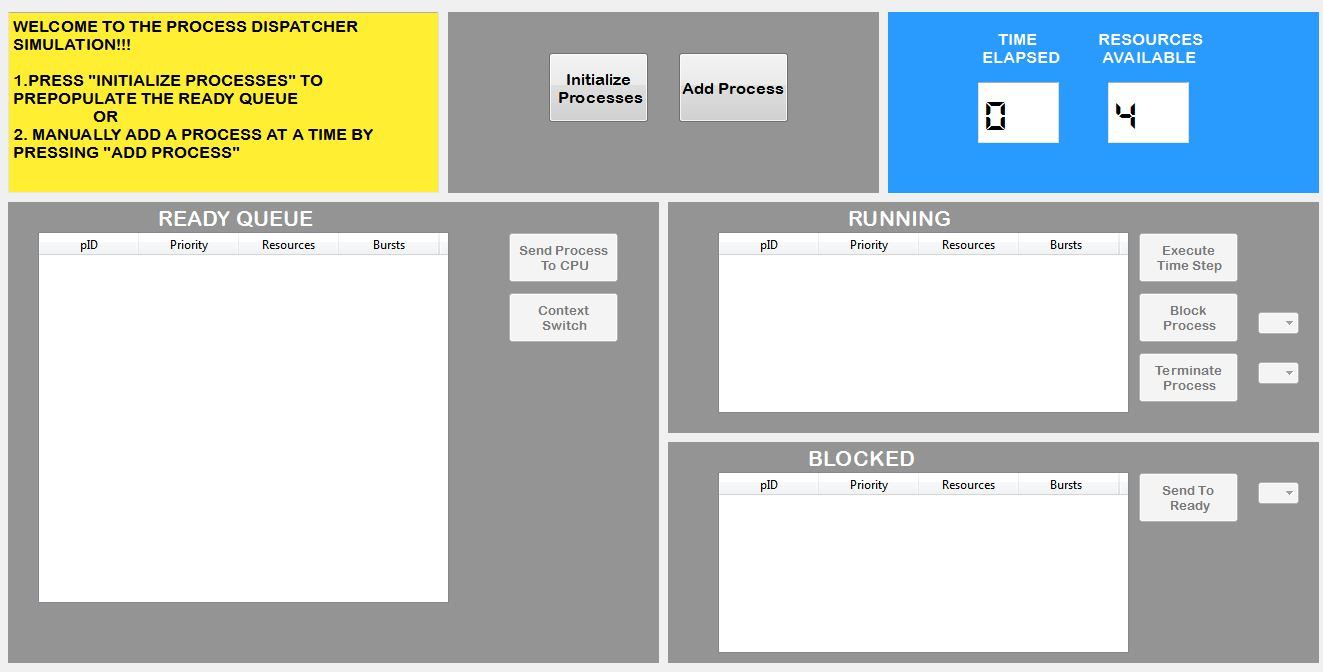
\includegraphics[width=\linewidth]{ss1.JPG}
 \caption{The entire GUI has six sections. The yellow message box, that gives the user usefull prompts on how to proceed. The blue ``Status Box'' that displays how many CPU resources are still available and how much time has elapsed}
\end{figure}


\newpage
\section*{{\underline{\huge {Screenshots :}}  }}
\begin{figure}[H]
 \centering
 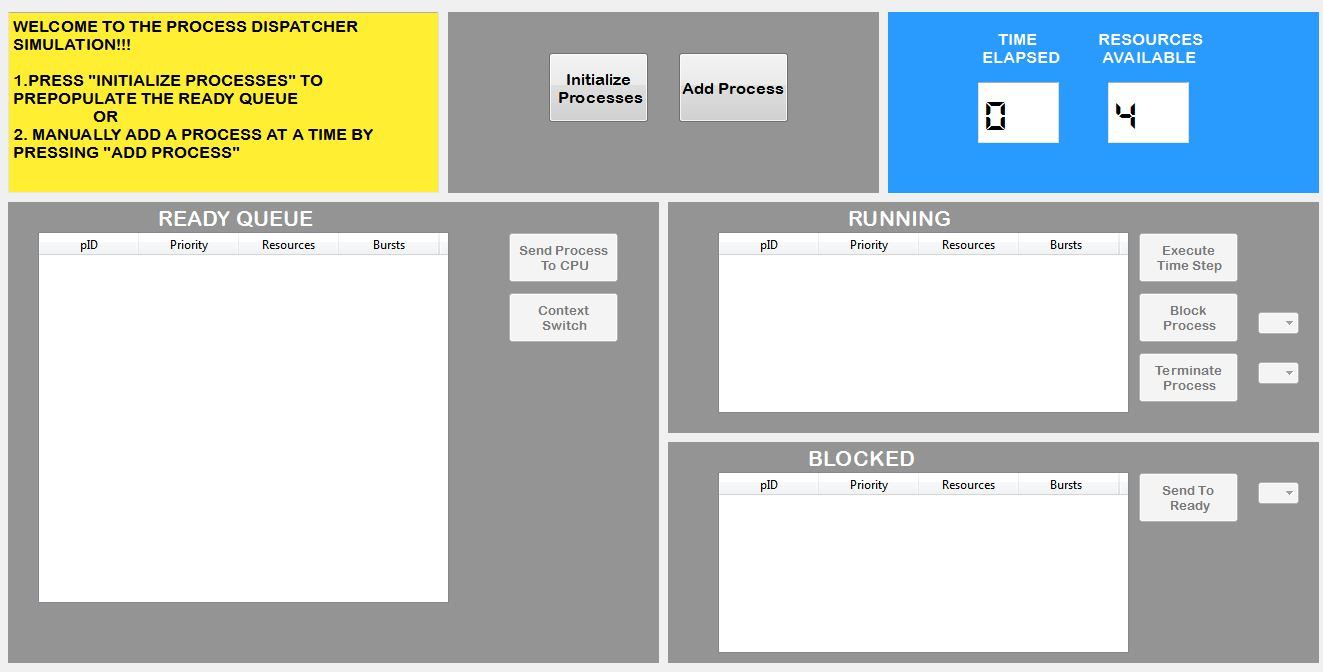
\includegraphics[width=\linewidth]{ss1.JPG}
 \caption{We will select ``Initialized Processes.}
\end{figure}

\begin{figure}[H]
 \centering
 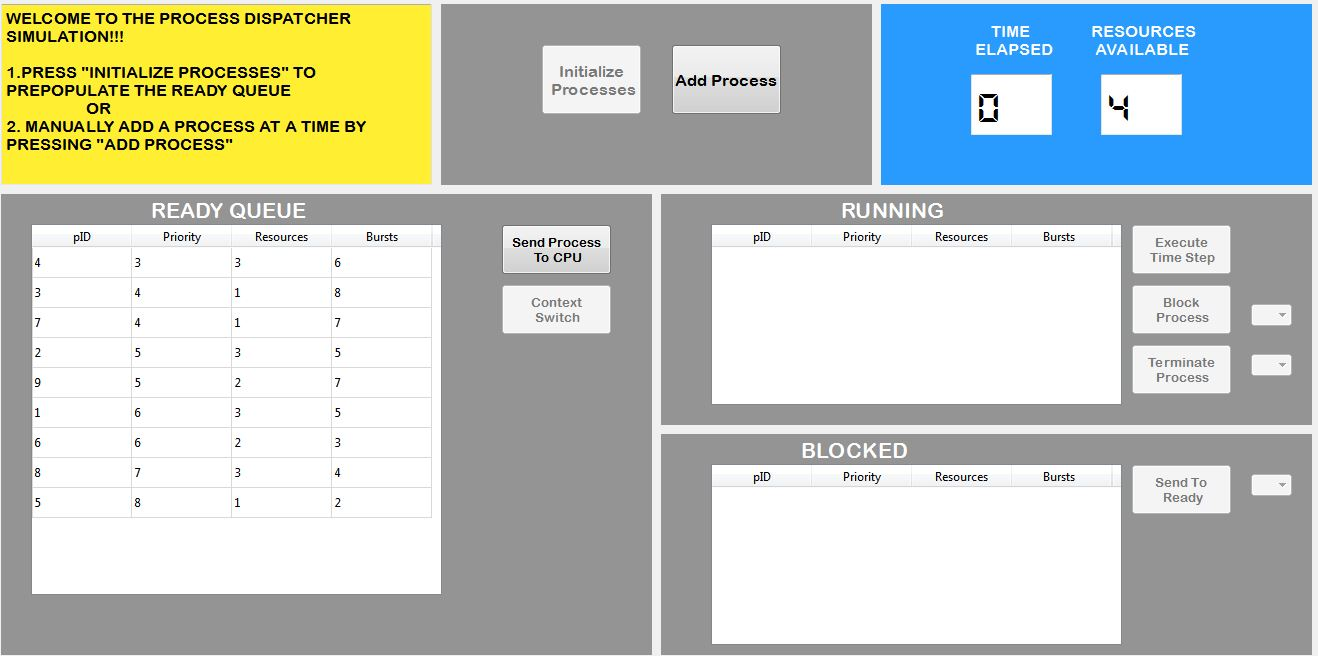
\includegraphics[height = 9 cm]{ss2.JPG}
 \caption{Processes are added to the ready queue.}
\end{figure}

\begin{figure}[H]
 \centering
 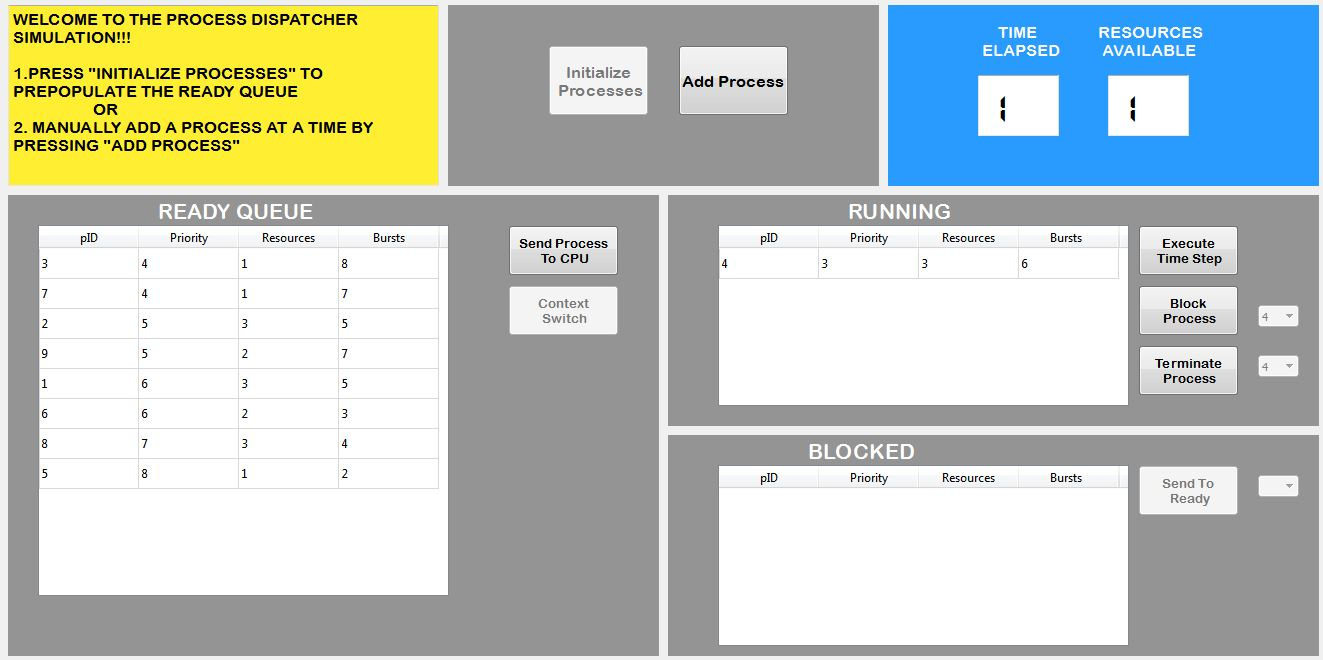
\includegraphics[height = 9 cm]{ss3.JPG}
 \caption{We send the process with the highest priority to the CPU.}
\end{figure}

\begin{figure}[H]
 \centering
 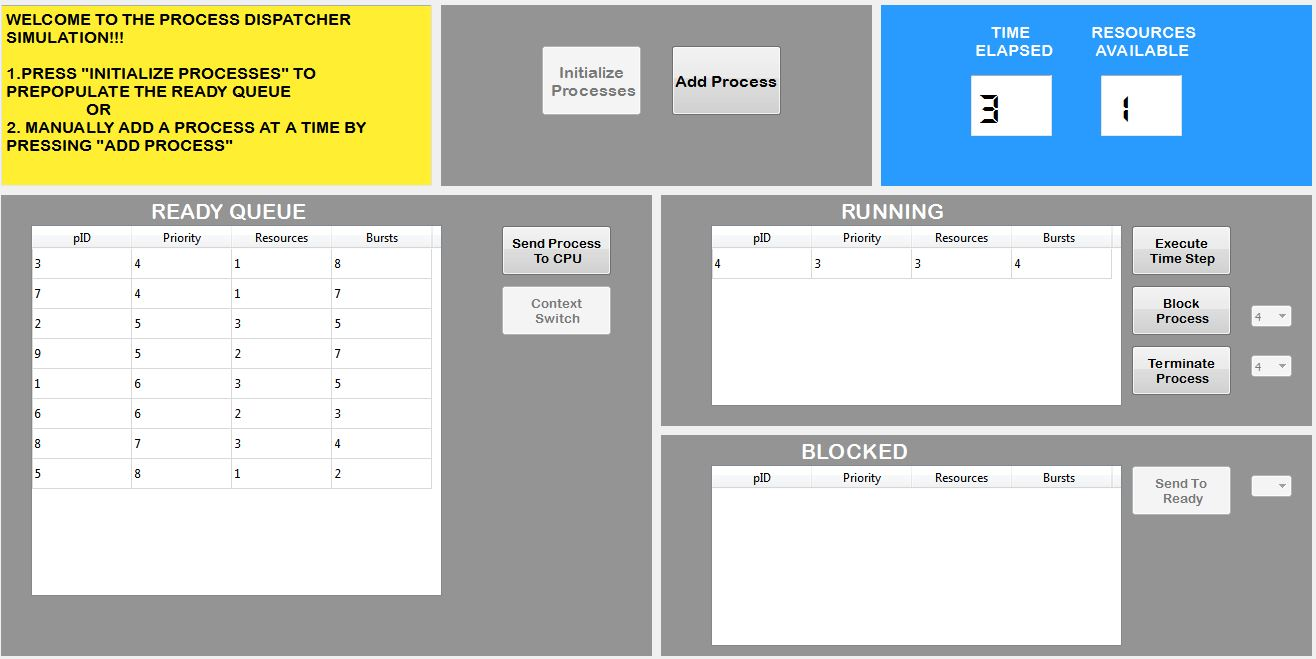
\includegraphics[height = 9 cm]{ss4.JPG}
 \caption{Execute time step.}
\end{figure}

\begin{figure}[H]
 \centering
 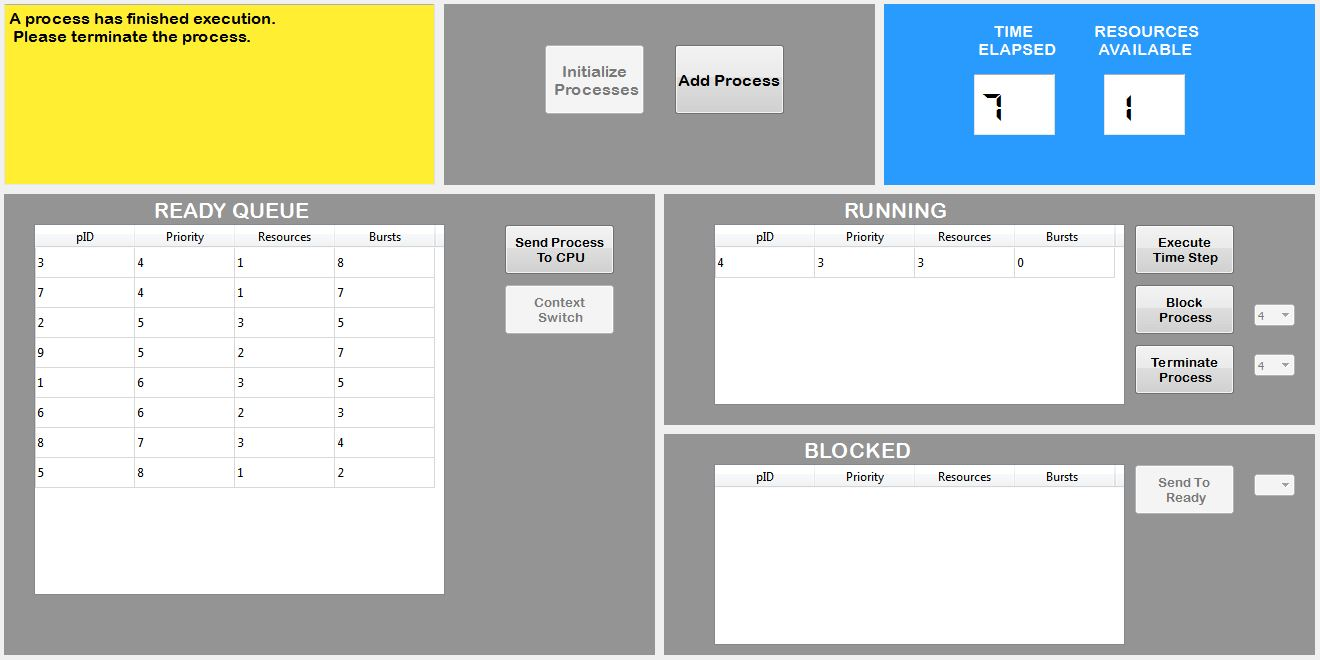
\includegraphics[height = 9 cm]{ss5.JPG}
 \caption{The process has finished executing (0 bursts). The user is prompted to terminate the process.}
\end{figure}

\begin{figure}[H]
 \centering
 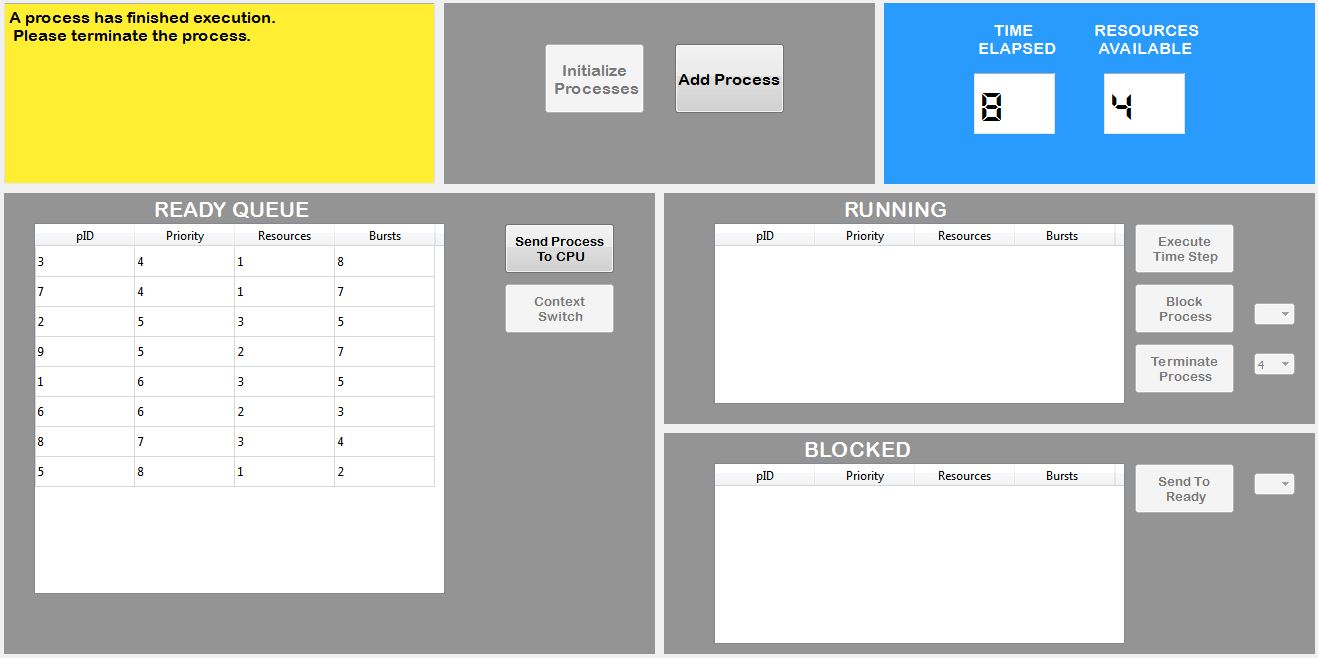
\includegraphics[height = 9 cm]{ss6.JPG}
 \caption{Process is terminated after pressing the ``Terminate Process'' button.}
\end{figure}

\begin{figure}[H]
 \centering
 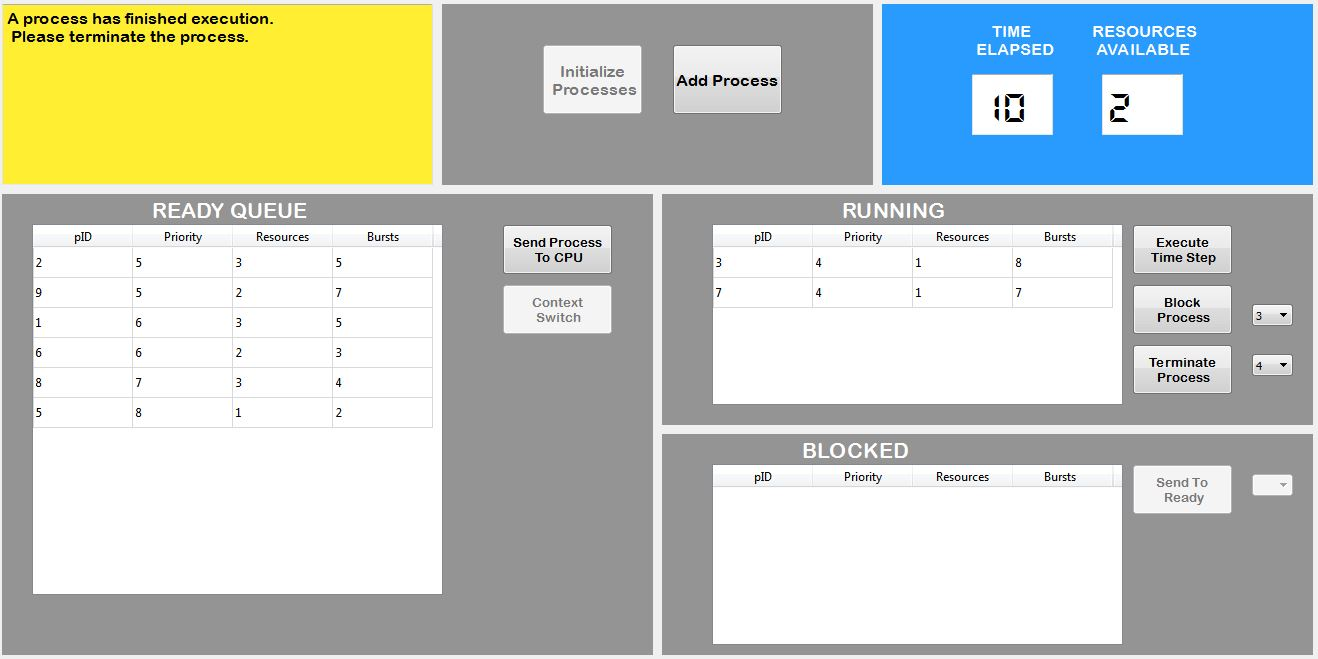
\includegraphics[height = 9 cm]{ss7.JPG}
 \caption{We have sent 2 processes for execution and will attempt to send a 3rd one.}
\end{figure}

\begin{figure}[H]
 \centering
 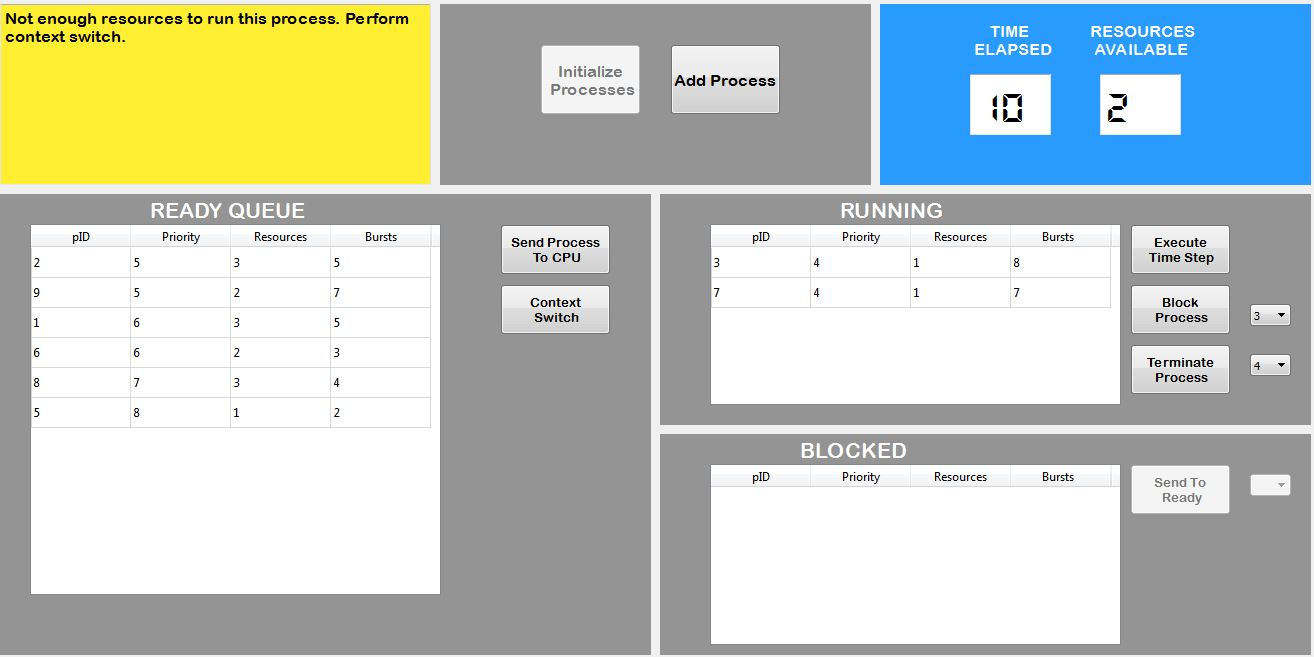
\includegraphics[height = 9 cm]{ss8.JPG}
 \caption{The user is alerted that there are not enough resources for process pID=2 to execute. The user is prompted to perform a context switch.}
\end{figure}

\begin{figure}[H]
 \centering
 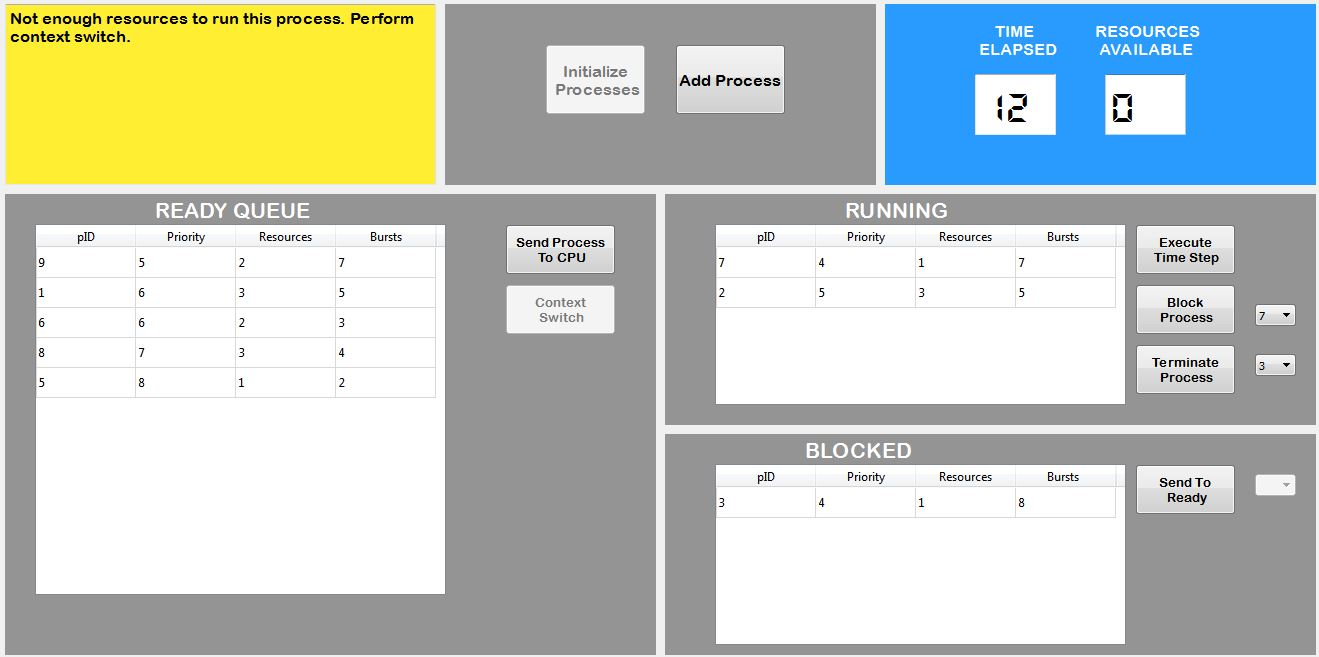
\includegraphics[height = 9 cm]{ss9.JPG}
 \caption{We performed a context switch. We blocked the older process and are now executing the process we just sent from the ready queue.}
\end{figure}

\begin{figure}[H]
 \centering
 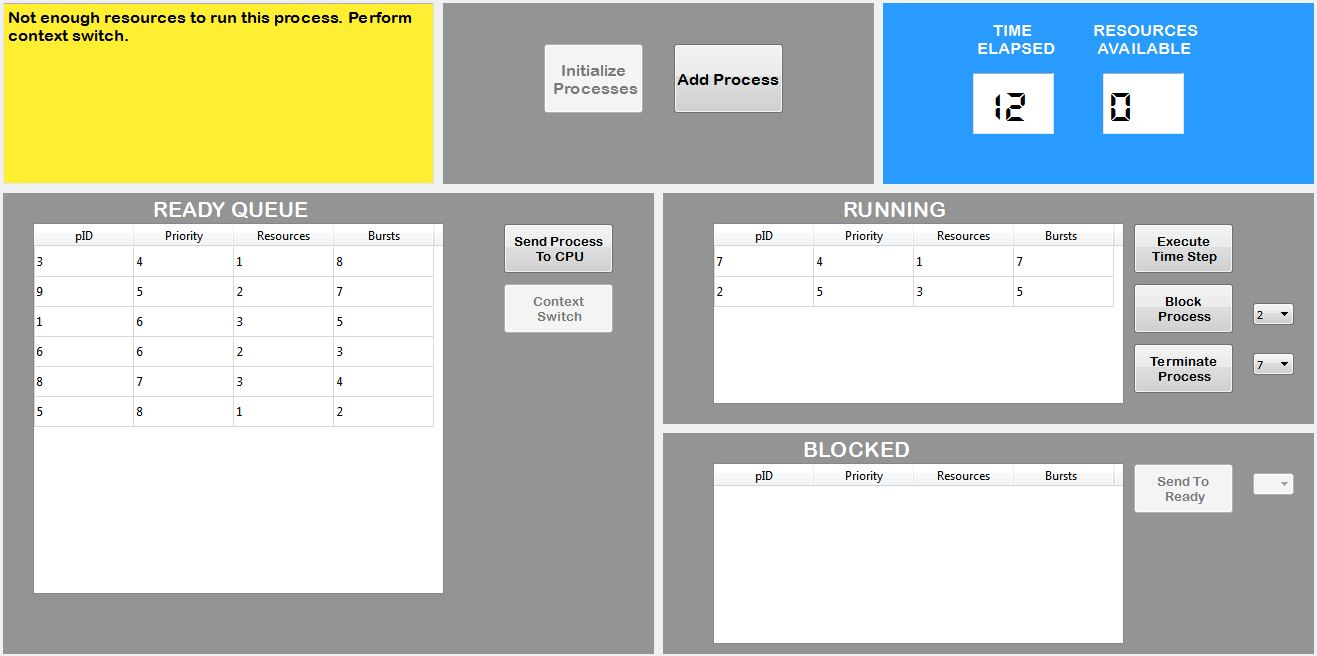
\includegraphics[height = 9 cm]{ss10.JPG}
 \caption{We sent the blocked process back to the ready queue. This does not affect the time elapsed.}
\end{figure}





%----------------------------------------------------------------------------------------
\end{document}
